% LaTeX source for book ``模形式初步'' in Chinese
% Copyright 2020  李文威 (Wen-Wei Li).
% Permission is granted to copy, distribute and/or modify this
% document under the terms of the Creative Commons
% Attribution 4.0 International (CC BY 4.0)
% http://creativecommons.org/licenses/by/4.0/

\chapter{\texorpdfstring{$L$}{L}-函数}
$L$-函数是模形式理论最核心也最深刻的不变量之一. 选定 $N, k$. 从 $M_k(\Gamma_1(N))$ 中的模形式 $f = \sum_{n \geq 0} a_n(f) q^n$ 出发, 可以构造 $L$-函数 $L(s,f) = \sum_{n \geq 1} a_n(f) n^{-s}$, 为此便须对 $(a_n(f))_{n \geq 0}$ 作初步的估计. 本章的主要结果是:
\begin{enumerate}
	\item Fourier 系数的初步估计 (\S\ref{sec:Fourier-estimate}), 由此推得 $L(s,f)$ 在 $\Re(s) \gg 0$ 时收敛并且全纯;
	\item Mellin 变换的基本理论 (\S\ref{sec:Mellin-Dirichlet});
	\item 当 $f$ 是正规化 Hecke 特征形式时, Euler 乘积
	\[ L(s,f) = \prod_{p: \text{素数}} \left( 1 - a_p(f) p^{-s} + \chi_f(p) p^{k-1-2s} \right)^{-1} \]
	在收敛范围内成立 (\S\ref{sec:L-fcn}), 其中 $\chi_f(p)$ 是 $f$ 对菱形算子 $\lrangle{p}$ 的特征值, 在 $p \mid N$ 时规定为 $0$;
	\item 对于任意尖点形式 $f \in S_k(\Gamma_1(N))$, 证明 $\Lambda_N(s,f) := N^{s/2} (2\pi)^{-s} \Gamma(s) L(s,f)$ 具有
	\begin{compactitem}
		\item 到整个 $\CC$ 上的全纯延拓, 在任意竖带上有界,
		\item 函数方程 $\Lambda(s,f) = \Lambda_N(k-s, W_N f)$, 这里 $W_N: S_k(\Gamma_1(N)) \to S_k(\Gamma_1(N))$ 是所谓的 Fricke 对合或 Atkin--Lehner 对合 (\S\ref{sec:L-cusp-form}).
	\end{compactitem}
\end{enumerate}

我们事实上将处理一般的 $f \in M_k(\Gamma_1(N))$, 这时 $\Lambda_N(s, f)$ 可能在 $s = 0, k$ 有单极点. 确立 $\Lambda_N(s,f)$ 解析性质的关键是应用 Mellin 变换表之为 $f$ 的某种周期积分, 这是 Hecke 的洞见. Euler 乘积和 $\Lambda_N(s,f)$ 的诸多解析性质是 $L$-函数的根本特征. Eisenstein 级数的 $L$-函数可以表达作所谓 Hecke 特征标的 $L$-函数, 但本书选择略过.

为了提供具体例子, 我们将穿插 $\vartheta$-级数, 平方和问题和凸性界的相关讨论.

本章参考了 \cite[\S 5.9]{DS05}. 关于凸性界的讨论是解析数论的课题; 关于 $L$-函数在这方面的角色及应用, 读者不妨参考 \cite{IS00,M07} 等相关文献.

\section{Fourier 系数的初步估计}\label{sec:Fourier-estimate}
考虑权为 $k \in \Z_{\geq 0}$ 的模形式. 眼下的目标是为尖点形式的 Fourier 系数提供最初步的估计.
\index{Fourier 系数}

以下选定余有限 Fuchs 群 $\Gamma$, 不失一般性假设 $\infty$ 是 $\Gamma$ 的尖点, 并考虑相应的 Fourier 展开. 记任意 $f \in M_k(\Gamma)$ 在该处的 Fourier 展开为 $\sum_{n \geq 0} a_n(f) q_r^n$, 其中
\begin{align*}
	r & := \min\left\{ t > 0 : \twomatrix{1}{t}{}{1} \in \Gamma \right\} \;\in \R_{>0}, \\
	q_r & := e^{2\pi i\tau/r}.
\end{align*}
由 \S\ref{sec:modular-form-general} 的讨论已知 $\twomatrix{1}{r}{}{1}$ 生成 $\Gamma \cap \twomatrix{1}{*}{}{1}$. 常用例子包括:
\begin{compactitem}
	\item $\Gamma = \Gamma(N)$, 这时 $r = N$;
	\item $\Gamma = \Gamma_1(N)$ 或 $\Gamma_0(N)$, 这时 $r = 1$.
\end{compactitem}

\begin{theorem}[E.\ Hecke]\label{prop:Hecke-bound}
	设 $f \in S_k(\Gamma)$, 则
	\begin{align*}
		|a_n(f)| & \ll n^{k/2}, \\
		\sum_{m \leq n} |a_m(f)|^2 & \ll n^k, \\
		\sum_{m \leq n} |a_m(f)| & \ll n^{(k+1)/2}.
	\end{align*}
%	估计中涉及的常数仅依赖于 $f$ 和 $\Gamma$.
\end{theorem}
\begin{proof}
	根据 Cauchy 积分公式, 置 $\tau = x+iy$, 固定 $y > 0$ 并取 $\epsilon := e^{-2\pi y/r} < 1$,
	\begin{align*}
		a_n(f) & = \frac{1}{2\pi i} \oint_{|q_r| = \epsilon} \left( \sum_{m \geq 1} a_m(f) q_r^m \right) q_r^{-n} \cdot \dfrac{\dd q_r}{q_r} \\
		& = \frac{1}{r} \int_0^r f(x+iy) \exp\left( -2\pi i \cdot \frac{n(x+iy)}{r} \right) \dd x \\
		\left(\text{取}\; y = \frac{1}{n}\right) \qquad & = \frac{e^{2\pi/r}}{r} \int_0^r f\left( x + \frac{i}{n} \right) e^{-2\pi inx/r} \dd x.
	\end{align*}
	命题 \ref{prop:Hecke-bound-prep} 表明 $B := \sup_{\tau \in \mathcal{H}} \left| f(\tau)\Im(\tau)^{k/2} \right|$ 有限, 故末项 $\ll n^{k/2}$. % 涉及的常数只和 $f$ 与 $\Gamma$ 有关.
	
	接着固定 $y > 0$, 考虑 $f$ 在横线 $\R + iy$ 上的 Fourier 展开
	\[ f\left( x + iy \right) =  \sum_{m \geq 1} a_m(f) e^{-2\pi my/r} e^{2\pi im x/r}. \]
	Parseval 公式 (定理 \ref{prop:Parseval}) 导致
	\[ \sum_{m \geq 1} |a_m(f)|^2 e^{-4\pi my/r}  = \dfrac{1}{r} \int_0^r |f(x + iy)|^2 \dd x \leq B y^{-k}. \]
	固定 $n \geq 1$, 以上估计给出
	\[ e^{-4\pi ny/r} \cdot \sum_{1 \leq m \leq n} |a_m(f)|^2 \leq \sum_{1 \leq m \leq n} |a_m(f)|^2 e^{-4\pi my/r} \leq \sum_{m=1}^\infty |a_m(f)|^2 e^{-4\pi my/r} \leq  B y^{-k}. \]
	和先前一样, 取 $y = 1/n$ 便是 $\sum_{m \leq n} |a_m(f)|^2$ 所需的估计. Cauchy--Schwarz 不等式给出 $\sum_{m \leq n} |a_m(f)|$ 的相应估计.
\end{proof}

若不要求 $f \in M_k(\Gamma)$ 为尖点形式, 但假定 $\Gamma$ 为同余子群, 则能得到稍弱的估计. 这时命题 \ref{prop:Eisenstein-complement} 将空间 $M_k(\Gamma)$ 分解成 $S_k(\Gamma)$ 和 Eisenstein 级数张成的 $\mathcal{E}_k(\Gamma)$ 两部分. 先前已经计算过一些 Eisenstein 级数的 Fourier 展开, 其系数的一般表达式虽然复杂, 终归是可算的.

\begin{theorem}\label{prop:Hecke-bound-cong}
	设 $\Gamma$ 为同余子群, $f \in M_k(\Gamma)$, 则 $|a_n(f)| \ll n^k$.
\end{theorem}
\begin{proof}
	无妨设 $k \geq 1$. 命题 \ref{prop:Eisenstein-complement} \footnote{该节构造的 Eisenstein 级数, 其 Fourier 展开和对应的直和分解可以通过解析延拓推及 $k = 1, 2$ 的情形, 细节比较复杂, 详阅 \cite[\S 7.2]{Mi89}.}
	给出 $M_k(\Gamma) = \mathcal{E}_k(\Gamma) \oplus S_k(\Gamma)$. 按照 \eqref{eqn:Eisenstein-general}, 如取 $N > 2$ 使得 $\Gamma \supset \Gamma(N)$, 则 $\mathcal{E}_k(\Gamma)$ 由 \S\ref{sec:Eisenstein-congruence-subgroup} 所定义的 Eisenstein 级数 $E_k^{\bar{v}} \in M_k(\Gamma(N))$ 的若干线性组合张成. 尖点形式部分可由定理 \ref{prop:Hecke-bound} 料理, 故处理 $f \in \mathcal{E}_k(\Gamma)$ 的情形足矣. 我们首先断言 $g := E_k^{\bar{v}}$ 对 $q_N := e^{2\pi i\tau/N}$ 作 Fourier 展开后的系数具有估计
	\[ |a_n(g)| \ll \begin{cases}
		n^{k-1}, & k \geq 3 \\
		n^{k-1+\epsilon}, & k =1,2
	\end{cases} \]
	其中 $\epsilon$ 是任意小的正数, $n \in \Z_{\geq 0}$. 根据定理 \ref{prop:Eisenstein-congruence-subgrp}, 仅须处理 $g = G_k^{\bar{v}}$ 的情形, 而且该定理还将问题进一步化约为对 $\sigma_{k-1}(n) := \sum_{d \mid n} d^{k-1}$ 验证上述估计, 这个数论问题是下一个引理的任务.
	
	回到 $f \in \mathcal{E}_k(\Gamma)$, 它是若干个 $E_k^{\bar{v}}$ 的线性组合, 故 $f$ 用 $q_N$ 展开后的 Fourier 系数也有如上估计, 但原来的问题是用 $q_r := e^{2\pi i\tau/r}$ 展开 $f$. 由 $\Gamma \cap \twomatrix{1}{*}{}{1} \supset \Gamma(N) \cap \twomatrix{1}{*}{}{1}$ 可知存在 $t \in \Z_{\geq 1}$ 使得 $N = tr$, 亦即 $q_r = q_N^t$; 由此导出 $a_n(f)$ 的相应估计.
\end{proof}

\begin{lemma}[见 {\cite[Theorem 4.7.3]{Mi89}} ]
	设 $k \in \Z_{\geq 1}$, 则函数 $\sigma_{k-1}$ 满足于
	\begin{gather*}
		\sigma_{k-1}(n) \ll \begin{cases}
			n^{k-1}, & k \geq 3 \\
			n^{1+\epsilon}, & k = 2 \\
			n^\epsilon, & k=1,
	\end{cases}\end{gather*}
	其中 $\epsilon$ 是任意正实数而 $n \in \Z_{\geq 1}$. 估计中涉及的常数依赖于 $k$.
\end{lemma}
\begin{proof}
	当 $k \geq 2$ 时,
	\[ \sigma_{k-1}(n) = \sum_{d \mid n} \left( \frac{n}{d} \right)^{k-1} = n^{k-1} \sum_{d \mid n} d^{-(k-1)}. \]
	
	若 $k \geq 3$, 上式小于等于 $n^{k-1} \zeta(k-1)$. 若 $k=2$, 上式写作
	\[ n \sum_{d \mid n} d^{-1} \leq n \left( 1 + \frac{1}{2} + \cdots + \frac{1}{n} \right) = n \left( \log n + \gamma + o(1) \right), \]
	其中 $\gamma$ 为 Euler 常数, 故右式由 $n^{1 + \epsilon}$ 控制.
	
	今探讨 $k = 1$ 情形. 设 $\epsilon > 0$, 取素因子分解 $n = \prod_{p: \text{素数}} p^{e_p}$. 易见
	\[ \sigma_0(n) = \prod_{p: \text{素数}} (e_p + 1), \quad \sigma_0(n)n^{-\epsilon} = \prod_{p: \text{素数}} \dfrac{e_p + 1}{p^{e_p \epsilon}}. \]
	注意到 $\log x < x$ 故 $e_p \epsilon \log 2 < 2^{e_p\epsilon} \leq p^{e_p \epsilon}$, 从而
	\begin{align*}
		\dfrac{e_p + 1}{p^{e_p \epsilon}} & = p^{-e_p \epsilon} + \dfrac{e_p}{p^{e_p \epsilon}} \leq 1 + \dfrac{e_p}{p^{e_p \epsilon}} \\
		& \leq 1 + \dfrac{1}{\epsilon\log 2} \leq \exp\left( \dfrac{1}{\epsilon \log 2} \right).
	\end{align*}
	当 $p \geq 2^{1/\epsilon}$ 时, 对之有更直截了当的估计
	\[ \dfrac{e_p + 1}{p^{e_p \epsilon}} \leq \dfrac{e_p + 1}{2^{e_p}} \leq 1. \]
	
	两则估计合并给出
	\[ \sigma_0(n) n^{-\epsilon} = \prod_p \dfrac{e_p + 1}{p^{e_p \epsilon}} \leq \prod_{p < 2^{1/\epsilon}} \exp\left( \dfrac{1}{\epsilon \log 2} \right) \leq \exp\left( \dfrac{2^{1/\epsilon}}{\epsilon\log 2} \right). \]
	明所欲证.
\end{proof}

\section{Mellin 变换与 Dirichlet 级数}\label{sec:Mellin-Dirichlet}
给定可测函数 $f: \R_{> 0} \to \CC$, 考虑含参数 $s \in \CC$ 的积分
\[ (\mathcal{M}f)(s) := \int_0^\infty f(t)t^s \dfrac{\dd t}{t}, \]
称之为 $f$ 的 \emph{Mellin 变换}, 收敛性是稍后的主题. 我们首先说明 Mellin 变换实质上是 Fourier 变换的某种解析延拓. Fourier 分析或曰调和分析其本质关乎拓扑群, 所以第一步是察知拓扑群的同构
\[ \exp: (\R, +) \longrightiso (\R_{>0}, \cdot), \quad x \mapsto t=e^x, \]
相应地
\begin{align*}
	\dd x & \longleftrightarrow \dd^\times t := \dfrac{\dd t}{t}:\; \text{拓扑群 $(\R_{>0}, \cdot)$ 上的不变测度} , \\
	[x \mapsto e^{sx}] & \longleftrightarrow [t \mapsto t^s]: \; \text{映至 $\CC^\times$ 的连续同态}, \quad s \in \CC.
\end{align*}
给定 $f: \R_{>0} \to \CC$, 定义 $g(x) = f(e^x): \R \to \CC$. 上述字典遂给出
\[ (\mathcal{M}f)(s) = \int_{\R_{>0}} f(t) t^s \dd^\times t = \int_{\R} g(x) e^{sx} \dd x \]
前提是所述积分存在. 当 $s = 2\pi i\xi \in i\R$ 时, 右式无非是 $g$ 的 Fourier (逆)变换 $\check{g}(\xi)$; 关于 Fourier 变换的约定详阅 \S\ref{sec:Poisson}.

以下处理积分变换 $\mathcal{M}$ 的收敛性, 并导出 Mellin 反演公式; 参阅 \cite[\S 1.29]{Ti86}.
\begin{proposition}\label{prop:Mellin-estimate}
	设 $a < b$ 为实数而可测函数 $f: \R_{> 0} \to \CC$ 满足估计
	\begin{align*}
		|f(t)| & \ll t^{-a}, \quad t \to 0, \\
		|f(t)| & \ll t^{-b}, \quad t \to \infty.
	\end{align*}
	\begin{enumerate}[(i)]
		\item 含参积分 $\mathcal{M}f(s) := \int_0^\infty f(t)t^s \dd^\times t$ 在 $a < \Re(s) < b$ 的紧子集上正规收敛 (见 \S\ref{sec:holomorphy}), 而且对于 $a < a' < b' < b$, 函数 $\mathcal{M}f(s)$ 在竖带 $a' \leq \Re(s) \leq b'$ 上有界, 对 $s$ 全纯.
		\item 假设 $f$ 连续, 并且进一步要求 $y \mapsto \mathcal{M}f(c + iy)$ 对每个 $a < c < b$ 皆属于 $L^1(\R)$, 或要求 $f$ 是局部有界变差函数, 则 Mellin 反演公式成立: 对如上实数 $c$ 和任意 $t > 0$,
		\begin{align*}
			f(t) & = \frac{1}{2\pi i} \int_{\Re(s) = c} t^{-s} \mathcal{M}(f)(s) \dd s \\
			& := \frac{1}{2\pi} \lim_{T \to +\infty} \int_{-T}^T \mathcal{M}(f)(c+iy) t^{-c-iy} \dd y.
		\end{align*}
	\end{enumerate}
\end{proposition}
\begin{proof}
	为了处理 (i), 先将 $\left| f(t)t^{s-1} \right|$ 的积分拆为 $\int_0^1$ 和 $\int_1^\infty$ 两段.	我们有
	\begin{align*}
		|f(t) t^{s-1}| & \ll t^{-a + \Re(s) - 1}, \quad 0 < t \leq 1, \\
		|f(t) t^{s-1}| & \ll t^{-b + \Re(s) - 1}, \quad t \geq 1.
	\end{align*}
	由之得到紧子集上的正规收敛性, 以及在 $\left\{ s \in \CC : a' \leq \Re(s) \leq b' \right\}$ 上的界. 进一步, 对于任何紧子集 $E \subset \R_{>0}$ 和 $K \subset \{s \in \CC: a < \Re(s) < b \}$, 基于对 $f$ 的估计, 函数族
	\[ \left\{ K \ni s \mapsto f(t) t^s \right\}_{t \in E} \]
	显然等度连续并且对 $s$ 全纯. 因之 $\mathcal{M}f(s)$ 的全纯性质是分析学的标准结果, 见命题 \ref{prop:integral-holomorphy}.
	
	接着来证明 (ii) 的反演公式. 命 $f_c(\eta) := f(e^\eta) e^{c\eta}$, 其中 $\eta \in \R$. 注意到
	\[ |f_c(\eta)| \ll \begin{cases}
		e^{(c-a)\eta}, & \eta \to -\infty \\
		e^{(c-b)\eta}, & \eta \to +\infty,
	\end{cases}\]
	所以 $a < c < b$ 确保 $f_c$ 是 $\R$ 上的速降函数. 换元 $t = e^\eta$ 给出
	\[ \mathcal{M}(f)(c + iy) = \int_{\R_{>0}} f(t) t^{c + iy} \dd^\times t = \int_{\R} f_c(\eta) e^{iy\eta} \dd\eta = (f_c)^\vee\left( \dfrac{y}{2\pi} \right); \]
	最后一个等号基于 \S\ref{sec:Poisson} 对 Fourier 变换的约定. 对 $f_c$ 应用 Fourier 反演 (定理 \ref{prop:Fourier-inversion}) 以导出
	\begin{align*}
		f_c(\eta) e^{-c\eta} & = e^{-c\eta} \lim_{T \to +\infty} \int_{-T}^T (f_c)^\vee(y) e^{-2\pi iy\eta} \dd y \\
		& = \dfrac{e^{-c\eta}}{2\pi} \lim_{T \to +\infty} \int_{-T}^T (f_c)^\vee\left( \dfrac{y}{2\pi} \right) e^{-iy\eta} \dd y \\
		& = \frac{1}{2\pi} \lim_{T \to +\infty} \int_{-T}^T \mathcal{M}(f)(c+iy) e^{-(c+iy)\eta} \dd y.
	\end{align*}
	重新以 $e^\eta = t$ 换元即所求.
\end{proof}

\begin{example}\label{eg:Gamma-Mellin}
	取 $f(t) = e^{-t}$, 那么以上估计中可取 $a=0$ 而 $b$ 任意大, 是故 $\mathcal{M}f(s)$ 在 $\Re(s) > 0$ 时收敛并给出 \S\ref{sec:Gamma} 讨论过的 $\Gamma$ 函数. 已知 $\Gamma(s)$ 可以延拓为 $\CC$ 上的亚纯函数, 而且根据熟知的复 Stirling 公式, 当 $c$ 限制在有界区间 $[c_1, c_2] \subset \R$ 时, 有一致的近似估计
	\begin{equation}\label{eqn:Gamma-vertical}
		|\Gamma(c+iy)| \sim \sqrt{2\pi} |y|^{c - \frac{1}{2}} e^{-\pi|y|/2}, \quad |y| \to \infty;
	\end{equation}
	特别地, $\Gamma(c + iy)$ 对 $|y|$ 速降, 故 Mellin 反演公式成立. 详见 \cite[3.12]{GW} 或 \cite[II.0.4]{Ten11}.
\end{example}

所谓 \emph{Dirichlet 级数}是形如 $\sum_{n \geq 1} a_n n^{-s}$ 的无穷级数, 其中 $a = (a_n)_{n=1}^\infty$ 是复数列而 $s$ 容许在 $\CC$ 的某个开子集中变动, 使得级数收敛. 在收敛的前提下, Dirichlet 级数对加法和乘法封闭
\begin{equation}\label{eqn:Dirichlet-convolution}\begin{aligned}
	\sum_{n \geq 1} a_n n^{-s} + \sum_{n \geq 1} b_n n^{-s} &= \sum_{n \geq 1} (a_n + b_n) n^{-s}, \\
	\sum_{n \geq 1} a_n n^{-s} \cdot \sum_{n \geq 1} b_n n^{-s} &= \sum_{n \geq 1} (a \star b)_n n^{-s},
\end{aligned}\end{equation}
此处定义 Dirichlet 卷积
\[ (a \star b)_n := \sum_{d \mid n} a_d b_{n/d}. \]

若 $a_1 = 1$ 而且 $a_n$ 满足
\[ \text{gcd}(n,m)=1 \implies a_{nm} = a_n a_m, \]
则形式的操作立刻给出 Euler 乘积
\[ \sum_{n \geq 1} a_n n^{-s} = \prod_{p: \text{素数}} \sum_{e \geq 0} a_{p^e} p^{-es}, \]
其严谨的成立条件则是 $\sum_{n \geq 1} |a_n| n^{-\Re(s)}$ 收敛 (定理 \ref{prop:Euler-product-general}); 这是诸位在 \S\ref{sec:Riemann-zeta} 学习 Riemann $\zeta$ 函数的 Euler 乘积时用过的技术.

\begin{exercise}
	证明当 $\Re(s) > 1$ 时 $\zeta(s)^{-1} = \sum_{n \geq 1} \mu(n) n^{-s}$, 此处 $\mu(n)$ 是数论中的 Möbius 函数.
\end{exercise}

\begin{exercise}\label{exo:Lambert}\index{Lambert 级数 (Lambert series)}
	对于复数列 $a = (a_n)_{n \geq 1}$, 定义 \emph{Lambert 级数}
	\[ \mathfrak{L}(q) := \sum_{n=1}^\infty \frac{a_n q^n}{1 - q^n}, \quad |q| < 1. \]
	证明若存在 $M \geq 0$ 使得 $|a_n| \ll n^M$, 则 $\mathfrak{L}(q)$ 收敛, 并且 $\mathfrak{L}(q) = \sum_{n=1}^\infty (a \star 1)_n q^n$, 其中 $1$ 代表常值列 $(1)_{n \geq 1}$. 依此对所有 $r \in \R$ 证明
	\[
		\sum_{n=1}^\infty \frac{n^r q^n}{1 - q^n} = \sum_{n=1}^\infty \sigma_r(n) q^n, \quad
		\sum_{n=1}^\infty \frac{\mu(n) q^n}{1 - q^n} = q.
	\]
\end{exercise}

\begin{theorem}\label{prop:Mellin-transform}
	设存在 $M \in \R$ 使得复数列 $(a_n)_{n \geq 1}$ 满足估计
	\begin{compactenum}[(a)]
		\item $|a_n| \ll n^M$, 或者
		\item $\sum_{m \leq n} |a_m| \ll n^{M+1}$,
	\end{compactenum}
	则以下性质成立.
	\begin{enumerate}[(i)]
		\item 设 $t \in \CC$, 则 $\tilde{f}(t) := \sum_{n \geq 1} a_n e^{-nt}$ 在 $\Re(t) > 0$ 时收敛, 而且当 $t \in \R$ 时
		\begin{align*}
			|\tilde{f}(t)| & \ll t^{-M - 1}, \quad t \to 0+ , \\
			|\tilde{f}(t)| & \ll e^{-t}, \quad t \to +\infty.
		\end{align*}
		\item Dirichlet 级数 $L(s) := \sum_{n \geq 1} a_n n^{-s} $ 在 $\Re(s) > M+1$ 时收敛. 若 $a > M+1$, 则 $L(s)$ 在区域 $\{s: \Re(s) \geq a\}$ 上一致有界.
		
		相对于参数 $t$, $s$, 无穷级数 $\tilde{f}(t)$ 和 $L(s)$ 皆在紧子集上正规收敛, 并且在收敛范围内分别对 $t,s$ 全纯.
		\item 当 $\Re(s) > M+1$ 时 $\mathcal{M}\tilde{f}(s)$ 由收敛积分定义, 对 $s$ 全纯, 此时
			\[ \Gamma(s) L(s) = (\mathcal{M}\tilde{f})(s) = \int_{\R_{>0}} \tilde{f}(t) t^s \dd^\times t; \]
			对于任意 $M + 1 < a < b < +\infty$, 上式作为 $s$ 的函数在竖带 $a \leq \Re(s) \leq b$ 上一致有界, 并且对 $|\Im(s)|$ 速降.
		\item 当实数 $c > M + 1$ 时, 对所有 $t > 0$ 皆有
			\[ \tilde{f}(t) = \frac{1}{2\pi i} \int_{\Re(s)=c} \Gamma(s) L(s) t^{-s} \dd s. \]
	\end{enumerate}
\end{theorem}

条件 $\sum_{m \leq n} |a_m| \ll n^{M + 1}$ 应理解为 $|a_m|$ 在平均意义下按 $n^M$ 增长. 断言 (iv) 的积分按命题 \ref{prop:Mellin-estimate} (ii) 的方法诠释.
\begin{proof}
	显然条件 (a) $\implies$ (b), 是故以下仅假定 (b).

	先处理 (ii). 命 $A_n := \sum_{m \leq n} |a_m|$, $b_n := n^{-\Re(s)}$. Abel 分部求和法蕴涵
	\begin{align*}
		\sum_{m=1}^n |a_m| m^{-\Re(s)} & = \sum_{m=1}^n (A_m - A_{m-1}) b_m, \quad A_0 := 0 \\
		& = \sum_{m=1}^n A_m b_m - \sum_{m=0}^{n-1} A_m b_{m+1} = \sum_{m=1}^n A_m \left( b_m - b_{m+1} \right) + A_n b_{n+1} \\
		& \leq \sum_{m=1}^n A_n \left| b_m - b_{m+1} \right| + A_n b_{n+1} .
	\end{align*}
	由于 $A_n \ll n^{M+1}$, 当 $\Re(s) > M+1$ 时 $A_n b_{n+1} \to 0$. 又由微分均值定理知 $\left| b_m - b_{m+1} \right|$ 可以用 $m^{-\Re(s)-1}$ 来控制, 故 $\sum_{m \geq 1} A_m \left| b_m - b_{m+1} \right|$ 在 $\Re(s) > M+1$ 时也收敛; 相关估计在区域 $\{s: \Re(s) \geq a\}$ 上是一致的. 按熟知的办法推导全纯性, 见命题 \ref{prop:sum-holomorphy}.

	回头处理 (i). 设 $t \in \R$. 条件 (b) 蕴涵 $|a_n| \ll n^{M+1}$, 故 $t > 0$ 时的收敛性是根审敛法的直接应用. 至于 $|\tilde{f}(t)|$ 的估计, 令 $Q := e^{-t}$. 在上述分部求和中改取 $b_m := Q^m$, 则
	\begin{align*}
		\sum_{m=1}^n |a_m| Q^m & = \sum_{m=1}^n A_m \left( b_m - b_{m+1} \right) + A_n b_{n+1} \\
		& = (1 - Q) \sum_{m=1}^n A_m Q^m + A_n Q^{n+1} \xrightarrow{n \to +\infty} (1 - Q) \sum_{m \geq 1} A_m Q^m \\
		& \ll (1 - Q) \sum_{m \geq 1} m^{M+1} Q^m.
	\end{align*}

	当 $t \to 0$ 时 $1 - Q = t + o(t)$, 由 $\sum_{m \geq 1} m^{M+1} Q^m$ 的大致公式 (参照命题 \ref{prop:automatic-holomorphy} 的证明) 可见
	\[ (1 - Q) \sum_{m \geq 1} m^{M+1} Q^m \ll (1 - Q)^{-M - 1} \sim t^{-M - 1}. \]
	这便给出 $t \to 0+$ 时的估计. 另一方面,
	\[ |\tilde{f}(t)| \leq \sum_{m \geq 1} |a_m| Q^m = Q \left( |a_1| + \sum_{m \geq 1} |a_{m+1}| Q^m \right). \]
	易见级数 $\sum_{m \geq 1} |a_{m+1}| \cdot |Q|^m$ 收敛而且对 $t$ 递减. 于是上式蕴涵 $t \to +\infty$ 时 $|\tilde{f}(t)| \ll Q$. 如是证得 (i).

	对于 (iii), $\mathcal{M}\tilde{f}(s)$ 的收敛范围和全纯性质是 (i) 和命题 \ref{prop:Mellin-estimate} 的结论. 形式地计算可得
	\begin{align*}
		\int_{\R_{>0}} \tilde{f}(t) t^s \dd^\times t &= \int_{\R_{>0}} \sum_{n \geq 1} a_n e^{-nt} t^s \dd^\times t \\
		& = \sum_{n \geq 1} a_n \int_{\R_{>0}} e^{-nt} t^s \dd^\times t \\
		(\text{换元}\; t \leadsto nt) \quad & = \sum_{n \geq 1} a_n n^{-s} \Gamma(s) = \Gamma(s) L(s),
	\end{align*}
	第三个等号用上了例 \ref{eg:Gamma-Mellin}; 为了确保收敛并交换积分与求和, 我们先在区域 $\Re(s) > \max\{0, M+1\}$ 上应用命题 \ref{prop:Mellin-estimate} 和 (i) 的估计, 以 Fubini 定理证成上述等式. 由于 $\mathcal{M}\tilde{f}(s)$ 和 $\Gamma(s) L(s)$ 都能延拓到 $\Re(s) > M + 1$ 上, 等式 $\Gamma(s) L(s) = \mathcal{M}\tilde{f}(s)$ 随之延拓.	在竖带 $a \leq \Re(s) \leq b$ 上的性状缘于 $L(s)$ 在竖带上一致有界和 $\Gamma$ 对 $|\Im(s)|$ 速降, 见 \eqref{eqn:Gamma-vertical}.
	
	最后, (iv) 直接导自 (iii) 和命题 \ref{prop:Mellin-estimate} 的 Mellin 反演公式.
\end{proof}

\begin{corollary}
	设数列 $(a_n)_{n=1}^\infty, (a^\dagger_n)_{n=1}^\infty$ 满足定理 \ref{prop:Mellin-transform} 的估计, 相应的 Dirichlet 级数分别记为 $L(s), L^\dagger(s)$, 则
	\[ \forall s, \; L(s) = L^\dagger(s) \iff \forall n, \; a_n = a^\dagger_n. \]
\end{corollary}
\begin{proof}
	根据定理 \ref{prop:Mellin-transform}, Dirichlet 级数 $L(s)$ 透过反演公式确定了 $\tilde{f}(t) = \sum_{n \geq 1} a_n Q^n$, 其中 $t > 0$ 而 $Q := e^{-t}$. 视 $\tilde{f}$ 为单位开圆盘 $\left\{ Q \in \CC : |Q| < 1 \right\}$ 上的全纯函数; 由于幂级数展开唯一, $(a_n)_{n=1}^\infty$ 也随之被确定了.
\end{proof}

由此可知 Dirichlet 级数 $L(s)$ 蕴藏了数列 $(a_n)_{n=1}^\infty$ 的一切信息.

\section{应用: 从 \texorpdfstring{$\theta$}{Theta} 级数到平方和问题}\label{sec:sum-of-squares}
对于一般的格都可以定义 $\vartheta$ 级数, 但本节只考虑最经典的 Jacobi $\vartheta$ 级数. 它以 $\tau \in \mathcal{H}$ 为参数, 定义为
\[ \vartheta(\tau) := \sum_{n \in \Z} q_2^{n^2}, \quad q_2 := e^{\pi i\tau}, \]
显见 $|q_2| < 1$, 故级数在紧集上正规收敛, 对 $\tau$ 全纯. 我们将研究与之相关的 Mellin 变换与模形式.

\begin{remark}\label{rem:Jacobi-form} \index{Jacobi 形式 (Jacobi form)}
	一般意义下的 $\vartheta$ 级数带两个变元
	\[ \vartheta(z;\tau) := \sum_{n \in \Z} q_2^{n^2} \eta^n, \quad q_2 := e^{\pi i\tau}, \; \eta := e^{2\pi i z}, \]
	其中 $(z,\tau) \in \CC \times \mathcal{H}$. 收敛与全纯毫无问题 (参阅 \S\ref{sec:holomorphy}), 而 $\vartheta(\tau) = \vartheta(0;\tau)$. 这是模形式理论中所谓 \emph{Jacobi 形式}的典型例子. 关于几何与表示论面向的讨论可见 \cite{Mum91}, 经典视角则可参照 \cite[第九章]{GW}; 这里的 $\vartheta(\tau;z)$ 对应于 \cite{GW} 的 $\vartheta_3$, 后者也是 Jacobi 原始的记法.
\end{remark}

\begin{theorem}[函数方程]\label{prop:theta-fcneq}
	我们有 $\vartheta(\tau + 2) = \vartheta(\tau)$. 对任意满足 $\Re(\eta) > 0$ 之复数 $\eta$, 记 $\sqrt{\eta}$ 为其在右半平面的平方根, 则
	\[ \vartheta(\tau) = \dfrac{1}{\sqrt{-i\tau}} \vartheta\left( \dfrac{-1}{\tau} \right). \]
\end{theorem}
\begin{proof}
	第一个断言缘于 $q_2(\tau + 2) = q_2(\tau)$. 第二个断言其等式两边对 $\tau$ 全纯, 于是仅须对 $\tau = i\eta \in i\R_{>0}$ 来验证. 首先定义含参数 $\eta > 0$ 的辅助函数
	\[ f_\eta(x) := e^{-\pi\eta x^2}, \quad x \in \R; \]
	它在 $\R$ 上是 $C^\infty$ 速降函数. 根据初等 Fourier 分析的一条标准结果 (如 \cite[Example 2.2.9]{Gra14} 配合 \eqref{eqn:Fourier-dilation}), 我们有
	\begin{equation}\label{eqn:f_eta-Fourier}
		(f_\eta)^\vee = \dfrac{1}{\sqrt{\eta}} f_{1/\eta}.
	\end{equation}
	于是 $(f_\eta)^\vee$ 也是 $\R$ 上的 $C^\infty$ 速降函数. 应用 Poisson 求和公式 (定理 \ref{prop:Poisson-sum}) 并代入 $\eta = \tau/i = -i\tau$ 和 \eqref{eqn:f_eta-Fourier}, 得到 $\vartheta(\tau)$ 等于
	\begin{align*}
		\sum_{n \in \Z} \exp\left(\pi i n^2 \tau \right) & = \sum_{n \in \Z} f_\eta(n) = \sum_{n \in \Z} (f_\eta)^\vee(n) \\
		& = \dfrac{1}{\sqrt{-i\tau}} \sum_{n \in \Z} \exp\left( \pi i \cdot \dfrac{-1}{\tau} \cdot n^2 \right).
	\end{align*}
	右式给出 $\dfrac{1}{\sqrt{-i\tau}} \vartheta\left(\dfrac{-1}{\tau}\right)$, 明所欲证.
\end{proof}

定义 $\R_{> 0}$ 上的函数
\begin{equation}\label{eqn:f-theta}\begin{aligned}
	f(t)  & := \dfrac{1}{2} \left(\vartheta(it)-1 \right) = \sum_{n \geq 1} e^{-\pi n^2 t}, \\
	\tilde{f}(t) & := f\left(\frac{t}{\pi}\right) = \sum_{n \geq 1} e^{-n^2 t}
\end{aligned}\end{equation}

置入定理 \ref{prop:Mellin-transform} 的框架, $\tilde{f}$ 对应于数列 $(a_n)_{n=1}^\infty$ 如下
\[ a_n := \begin{cases}
	1, & n: \text{平方数} \\
	0, & n: \text{非平方数}.
\end{cases} \]
显然有 $\sum_{m \leq n} a_n \leq \sqrt{n}$. 这相当于说定理 \ref{prop:Mellin-transform} 所需的估计对 $M = -\frac{1}{2}$ 成立. 因此 Mellin 变换 $\mathcal{M}\tilde{f}(s)$ 在 $\Re(s) > \frac{1}{2}$ 时收敛并且对 $s$ 全纯.

\begin{theorem}[B.\ Riemann]\label{prop:zeta-fcn-Mellin}
	定义 $f$ 如 \eqref{eqn:f-theta}. Mellin 变换 $\mathcal{M}f(s)$ 在 $\Re(s) > \frac{1}{2}$ 时收敛并给出 $s$ 的全纯函数. 它具有在 $\CC$ 上的亚纯延拓, 其唯一极点在 $s=0, \frac{1}{2}$ 处, 分别是留数为 $-\frac{1}{2}$ 和 $\frac{1}{2}$ 的单极点, 并且满足函数方程
	\[ \mathcal{M}f(s) = \mathcal{M}f\left( \frac{1}{2} - s \right). \]
	进一步, $\mathcal{M}f(s) = \pi^{-s} \Gamma(s) \zeta(2s)$.
\end{theorem}
\begin{proof}
	关于 $\mathcal{M}f(s)$ 的收敛范围, 全纯性等显然和 $\mathcal{M}\tilde{f}(s)$ 相同; 实际上
	\[ \mathcal{M}\tilde{f}(s) = \int_{\R_{>0}} f\left( \frac{t}{\pi} \right) t^s \dd^\times t = \pi^s \int_{\R_{>0}} f(t) t^{-s} \dd^\times t = \pi^s \mathcal{M}f(s). \]
	由之前观察遂知 $\mathcal{M}f(s)$, $\mathcal{M}\tilde{f}(s)$ 在 $\Re(s) > \frac{1}{2}$ 时收敛并全纯.
	
	以下将同步导出亚纯延拓和函数方程. 首先将 $\mathcal{M}f(s)$ 拆分为
	\[ \int_0^1 f(t) t^s \dd^\times t + \int_1^\infty f(t) t^s \dd^\times t. \]

	回忆命题 \ref{prop:Mellin-estimate} 证明可知 $\int_1^\infty$ 对任何 $s$ 都收敛, 而 $\int_0^1$ 的收敛范围是 $\Re(s) > \frac{1}{2}$. 对积分 $\int_0^1$ 施行换元 $u := \frac{1}{t}$: 注意到 $\frac{\dd u}{u} = - \frac{\dd t}{t}$ 并应用定理 \ref{prop:theta-fcneq}, 得出 $\int_0^1 f(t) t^s \dd^\times t$ 等于
	\begin{multline*}
		\dfrac{1}{2} \int_0^1 \left( \dfrac{1}{\sqrt{t}} \vartheta\left( \dfrac{i}{t} \right) - 1 \right) t^s \dd^\times t
		= \dfrac{1}{2} \int_1^\infty \left( \sqrt{u} \vartheta\left( iu \right) - 1 \right) u^{-s} \dd^\times u \\
		= \int_1^\infty \dfrac{\vartheta(iu) - 1}{2} \cdot u^{-s + \frac{1}{2}} \dd^\times u \; + \; \dfrac{1}{2} \left( \int_1^\infty u^{-s + \frac{1}{2}} \dd^\times u - \int_1^\infty u^{-s} \dd^\times u \right) \\
		= \int_1^\infty f(u) u^{\frac{1}{2} - s} \dd^\times u \; - \; \dfrac{1}{2} \left( \dfrac{1}{\frac{1}{2} - s} + \dfrac{1}{s} \right).
	\end{multline*}

	综上, 当 $\Re(s) > \frac{1}{2}$ 时
	\[ \mathcal{M}f(s) = \int_1^\infty f(t) t^s \dd^\times t + \int_1^\infty f(t) t^{\frac{1}{2} - s} \dd^\times t - \dfrac{1}{2} \left( \dfrac{1}{\frac{1}{2} - s} + \dfrac{1}{s} \right). \]
	定理 \ref{prop:Mellin-transform} 蕴涵 $f(t)$ 在 $t \to +\infty$ 时按指数衰减, 因而积分 $\int_1^\infty f(t) t^s \dd^\times t$ 和 $\int_1^\infty f(t) t^{\frac{1}{2} - s} \dd^\times t$ 对所有 $s \in \CC$ 皆收敛且全纯, 故右式是 $s \in \CC$ 的亚纯函数, 其极点的描述正与断言相符, 并且右式显然对 $s \leftrightarrow \frac{1}{2} -s$ 对称, 由此同时导出 $\mathcal{M}f$ 的亚纯延拓, 极点信息与函数方程.

	将 $\tilde{f}(t) = \sum_{n \geq 1} e^{-n^2 t}$ 代入定理 \ref{prop:Mellin-transform}, 可知当 $\Re(s) > \frac{1}{2}$ 时
	\[ \Gamma(s) \sum_{n \geq 1} n^{-2s} = \mathcal{M}\tilde{f}(s) = \pi^s \mathcal{M}f(s), \]
	整理后得到 $\mathcal{M}f(s) = \pi^{-s} \Gamma(s) \zeta(2s)$; 根据亚纯延拓, 此式对所有 $s \in \CC$ 成立. 明所欲证.
\end{proof}

以上证明未动用 $\zeta(s) = \sum_{n \geq 1} n^{-s}$ 的任何已知性质, 它实际给出了 $\zeta$ 的亚纯延拓, 极点描述与函数方程的另一套证明. 这一论证也出自 Riemann.

我们将目光转向数论中的平方和问题. 符号稍易, 命
\[ \theta(\tau) := \vartheta(2\tau) = \sum_{n \in \Z} q^{n^2}, \quad q := e^{2\pi i\tau}. \]

函数 $\theta$ 具有数论上的兴味: 基于幂级数在收敛范围 $|q| < 1$ 内的乘法, 对任意 $m \in \Z_{\geq 1}$ 皆有
\[ \theta(\tau)^m = \sum_{n \geq 0} r_m(n) q^n, \]
其中的系数
\[ r_m(n):= \left| \left\{ (n_i)_{i=1}^k \in \Z^k : n_1^2 + \cdots + n_k^2 = m \right\}\right| \]
是整数写作 $m$ 个平方和的表法个数. 且先介绍一个粗糙的估计. 记 $\R^m$ 的标准范数为 $\|\cdot\|$, 而 $\mathbb{B}^m := \{ x \in \R^m: \|x\| \leq 1 \}$ 为单位闭球.

\begin{proposition}\label{prop:r-estimate}
	定义 $R_m(n) :=\sum_{h \leq n} r_m(h)$, 则
	\[ \lim_{n \to \infty} \dfrac{R_m(n)}{n^{ \frac{m}{2} }} = \mes(\mathbb{B}^m) = \dfrac{\pi^{\frac{m}{2}}}{\Gamma\left( 1 + \frac{m}{2} \right)}, \]
	而且 $r_m(n) \ll n^{m/2}$, 估计中的常数依赖于 $m$.
\end{proposition}

关于 $R_m(n)$ 或其种种变体的估计称为 \emph{Gauss 圆内整点问题}.

\begin{proof}
	不妨设 $n > m$, 这时 $R_m(n) = \left| \sqrt{n} \cdot \mathbb{B}^m \cap \Z^m \right| \geq 1$; 对每个 $x \in \sqrt{n} \cdot \mathbb{B}^m \cap \Z^m$ 作相应的方块 $x + [0,1]^m$, 诸方块内部无交, 其并则记为 $\mathcal{R}$, 则 $\mes(\mathcal{R}) = R_m(n)$. 我们断言
	\[ (\sqrt{n} - \sqrt{m}) \cdot \mathbb{B}^m \subset \mathcal{R} \subset (\sqrt{n} + \sqrt{m}) \cdot \mathbb{B}^m. \]
	首先, 若 $y \in x + [0,1]^n$ 则三角不等式蕴涵 $\|y\| \leq \|x\| + \sqrt{n}$, 由此得到第二个 $\subset$. 若 $\|y\| \leq \sqrt{n} - \sqrt{m}$, 则 $x := \left( \lfloor y_i \rfloor \right)_{i=1}^m$ 满足于 $y \in x + [0,1]^n$, 而 $\|x\| \leq \|y\| + \sqrt{m} \leq \sqrt{n}$, 由此得到第一个 $\subset$. 下图是 $m=2, n=9$ 的情形:
	\begin{center}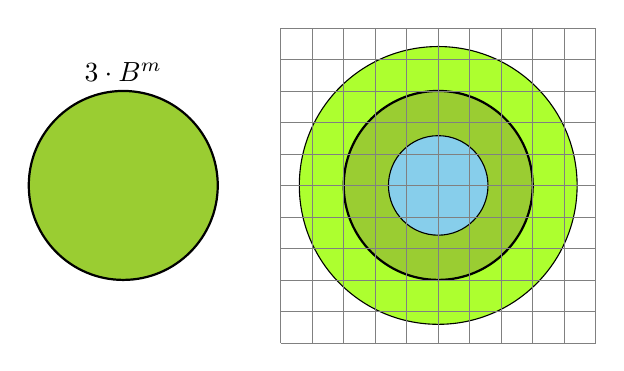
\begin{tikzpicture}[scale=0.4, baseline=(O)]
		\filldraw[fill=GreenYellow] (0,0) circle[radius=4.41];	% 3 + sqrt(2), approximately 4.41
		\filldraw[thick, fill=YellowGreen] (0,0) circle[radius=3];
		\filldraw[fill=SkyBlue] (0,0) circle[radius=1.58];	% 3 - sqrt(2), approximately 1.58
		\draw[step=1, gray, very thin] (-5,-5) grid (5,5);
		\coordinate (O) at (0,0);
		\filldraw[thick, fill=YellowGreen] (-10, 0) circle[radius=3];
		\node at (-10, 3) [above] {$3\cdot \mathbb{B}^m$};
	\end{tikzpicture} \end{center}
	比较体积并取极限 $n \to \infty$ 即得第一式; 关于 $\mathbb{B}^m$ 体积的公式是熟知的.	由于 $r_m(n) \leq R_m(n)$, 随之得到上界.
\end{proof}

焦点转回 $\theta$ 本身. 定理 \ref{prop:theta-fcneq} 化为
\[ \theta(\tau + 1)^m = \theta(\tau)^m, \quad \theta\left( \tau \right)^m = \dfrac{1}{\left(\sqrt{-2i\tau}\right)^m} \theta\left( \dfrac{-1}{4\tau} \right)^m. \]

考虑 $\SL(2,\Q)$ 的元素
\[ T := \twobigmatrix{1}{1}{}{1}, \quad V_4 := \frac{1}{2} \twobigmatrix{}{-1}{4}{}; \qquad  V_4^2 = \twobigmatrix{-1}{}{}{-1}. \]
当 $m = 2k$ 时 $(\sqrt{-2i\tau})^{-m} = (-2i\tau)^{-k} = i^k (2\tau)^{-k}$, 上式可改写作
\begin{equation}\label{eqn:theta-V4}
	\theta^{2k} = \theta^{2k} \modact{k} T, \quad \theta^{2k} = i^k \theta^{2k} \modact{k} V_4 = i^k \theta^{2k} \modact{k} \twomatrix{}{-1}{4}{}.
\end{equation}
这暗示 $\theta^{2k}$ 有望成为权 $k$ 的模形式; 实际上, 相应的离散子群可以取为同余子群 $\Gamma_0(4)$, 并且对 $\Gamma_0(4)/\Gamma_1(4) = (\Z/4\Z)^\times$ 到 $\CC^\times$ 的某个同态具有等变性. 下面就来补全细节.

\begin{lemma}\label{prop:Gamma_0(4)-gen}
	同余子群 $\Gamma_0(4)$ 在 $\PSL(2,\R)$ 中的像由 $T$ 和 $\tilde{T} := V_4 T V_4^{-1} = \twomatrix{1}{}{4}{1}$ 生成.
\end{lemma}
\begin{proof}
	设 $\gamma = \twomatrix{a}{b}{4c}{d} \in \Gamma_0(4)$. 我们对 $a^2 + b^2$ 递归来说明 $\pm\gamma$ 能由 $T, \tilde{T}$ 表出. 设 $a^2 + b^2 = 1$; 假若 $a=0$, 此时 $\det\gamma = -4bc$ 不可能为 $1$; 若 $b=0$ 则 $\gamma = \pm \twomatrix{1}{}{4m}{1} = \pm\tilde{T}^m$. 以下考虑 $a^2 + b^2 > 1$ 情形; 此时 $b \neq 0$, 否则 $\det\gamma = 1$ 将蕴涵 $|a|=1$, 与 $a^2 + b^2 > 1$ 矛盾. 又由 $a \notin 2\Z$ 可知 $|a| \neq 2|b|$. 下面应用一则初等的观察: 设 $x,y \in \R$ 满足 $0 < |x| < 2|y|$, 那么分析正负号可知 $|y+x| < |y|$ 或 $|y-x| < |y|$ 必居其一.
	\begin{enumerate}
		\item 若 $|a| < 2|b|$, 上述观察给出 $|a+b| < |b|$ 或 $|a-b| < |b|$; 此时分别以 $\gamma T^{\pm 1}$ 代 $\gamma$ 来缩小 $a^2 + b^2$.
		\item 若 $|a| > 2|b|$ 则 $|4b| < 2|a|$, 上述观察给出 $|a+4b| < |a|$ 或 $|a-4b| < |a|$; 此时分别以 $\gamma \tilde{T}^{\pm 1}$ 代 $\gamma$ 来缩小 $a^2 + b^2$.
	\end{enumerate}
	明所欲证.
\end{proof}

定义群同态
\begin{align*}
	\chi: (\Z/4\Z)^\times & \longrightarrow \CC^\times \\
	\pm 1 \bmod 4\Z & \longmapsto \pm 1.
\end{align*}

\begin{lemma}\label{prop:theta-modular-invariance}
	取 $\chi$ 如上, 设 $k \in \Z_{\geq 1}$, 则对所有 $\gamma = \twomatrix{a}{b}{c}{d} \in \Gamma_0(4)$ 都有 $\theta^{2k} \modact{k} \gamma = \chi(d)^k \theta^{2k}$. 作为特例, 当 $\gamma \in \Gamma_1(4)$ 时 $\theta^{2k} \modact{k} \gamma = \theta^{2k}$.
\end{lemma}
\begin{proof}
	取 $\gamma = \twomatrix{-1}{}{}{-1}$ 则 $\theta^{2k} \modact{k} \twomatrix{-1}{}{}{-1} = (-1)^k \theta^{2k} = \chi(-1)^k \theta^{2k}$. 取 $\gamma = T$ 则 $\chi(d)=1$ 而 $\theta^{2k} \modact{k} T = \theta^{2k}$. 最后取引理 \ref{prop:Gamma_0(4)-gen} 的 $\gamma = \tilde{T}$, 则 $\chi(d) = 1$ 而
	\[ \theta^{2k} \modact{k} \tilde{T} = \theta^{2k} \modact{k} V_4 \modact{k} T \modact{k} V_4^{-1} = \theta^{2k}. \]
	根据引理 \ref{prop:Gamma_0(4)-gen}, 这三个元素生成 $\Gamma_0(4)$. 证毕.
\end{proof}

\begin{proposition}
	设 $k \in \Z_{\geq 1}$, 则 $\theta^{2k} \in M_k\left( \Gamma_0(4), \chi^k \right)$. 它在尖点 $\infty$ 处取值为 $1$.
\end{proposition}
\begin{proof}
	首先证明 $\theta^{2k} \in M_k(\Gamma_0(4), \chi^k)$. 基于命题 \ref{prop:automatic-holomorphy-cong}, 再配合引理 \ref{prop:theta-modular-invariance} 提供的 $(\Gamma_1(4), \chi)$-等变性, 仅须验证 $\theta^{2k}$ 在尖点 $\infty$ 处的 Fourier 展开
	\[ \theta(\tau)^{2k} = \sum_{n \geq 0} r_{2k}(n) q^n \]
	中的系数 $r_{2k}(n)$ 至多按多项式增长, 然而这由命题 \ref{prop:r-estimate} 确保. 显然 $r_{2k}(0) = 1$.
\end{proof}

当 $h$ 为正奇数时, $\theta^h$ 可以用\emph{半整权模形式}的理论来解释. 特别地, $\theta$ 是权为 $\frac{1}{2}$ 的模形式. Serre 和 Stark 的一个著名定理断言所有权为 $\frac{1}{2}$, 级为某个算术子群 $\Gamma \subset \SL(2,\Z)$ 的模形式都可以写作 $\theta_{u,v} := \sum_{n \in \Z} q^{u(n+v)^2}$ 的线性组合, 以此观之, $\theta$ 级数也就穷尽了权为 $\frac{1}{2}$ 的模形式. 一般的半整权 $h + \frac{1}{2}$ 模形式和整权 $2h$ 模形式之间则有深刻的对应关系, 这是由志村五郎, Kohnen, Gelbart, Piatetski-Shapiro 和 Waldspurger 等人奠基的工作. \index{moxingshi!半整权 (of half-integral weight)}

我们业已将 $k$ 平方和的表法数 $r_k(n)$ 诠释为模形式 (容许半整权) 的 Fourier 系数. 牛刀小试, 首先琢磨 $r_4(n)$. 回忆定义 \ref{def:E2} 构造的全纯函数 $E_2, G_2$ 以及
\[ \mathcal{G}_2(\tau) := \dfrac{G_2(\tau)}{-8\pi^2} = \dfrac{E_2(\tau)}{-24} = -\dfrac{1}{24} + \sum_{n=1}^\infty  \sigma_1(n) q^n. \]
等式 \eqref{eqn:E2-fcneq} 蕴涵 $\tau^{-2} \mathcal{G}_2(-1/\tau) = \mathcal{G}_2(\tau) - (4\pi i\tau)^{-1}$, 它不是模形式, 但实解析函数 $\mathcal{G}^*_2(\tau) := \mathcal{G}_2(\tau) + \dfrac{1}{8\pi\Im(\tau)}$ 则满足于 $\gamma \in \SL(2,\Z) \implies \mathcal{G}^*_2 \modact{2} \gamma = \mathcal{G}^*_2$ (练习 \ref{exo:G2}).

\begin{exercise}
	对所有 $N \in \Z_{\geq 1}$ 证明 $\mathcal{G}_2(\tau) - N\mathcal{G}_2(N\tau) = \mathcal{G}^*_2(\tau) - N\mathcal{G}^*_2(N\tau)$ 属于 $M_2(\Gamma_0(N))$.

	\begin{hint} 可应用命题 \ref{prop:automatic-holomorphy-cong} 和 \ref{prop:oldform}. \end{hint}
\end{exercise}

基于以上练习, $M_2(\Gamma_0(4))$ 含有元素
\begin{align*}
	\mathcal{G}_2(\tau) - 2\mathcal{G}_2(2\tau) & = \dfrac{1}{24} + q + q^2 + \cdots, \\
	\mathcal{G}_2(2\tau) - 2\mathcal{G}_2(4\tau) & = \dfrac{\mathcal{G}_2(\tau) - 4\mathcal{G}_2(4\tau)}{2} - \dfrac{\mathcal{G}_2(\tau) - 2\mathcal{G}_2(2\tau)}{2} \\
	& = \dfrac{1}{24} + 0 \cdot q + q^2 + \cdots. 
\end{align*}
观察 Fourier 展开前两项可知两者线性无关. 因为维数公式给出 $\dim_{\CC} M_2(\Gamma_0(4)) = 2$ (例 \ref{eg:dimension-Gamma04}), 以上两者给出 $M_2(\Gamma_0(4))$ 的一组基. 容易算出 $r_4(1)=8$; 代入 $\theta(\tau)^4 = 1 + 8q + \cdots \in M_2(\Gamma_0(4))$, 登时解出
\[ \theta(\tau)^4 = 8 \left( \mathcal{G}_2(\tau) - 2\mathcal{G}_2(2\tau) \right) + 16\left( \mathcal{G}_2(2\tau) - 2\mathcal{G}_2(4\tau) \right) = 8(\mathcal{G}_2(\tau) - 4\mathcal{G}_2(4\tau)). \]

\begin{theorem}[C.\ G.\ J.\ Jacobi]
	对于 $n \in \Z_{\geq 1}$, 我们有 $r_4(n) = 8 \sum_{\substack{d \mid n \\ 4 \nmid d}} d$.
\end{theorem}
\begin{proof}
	鉴于 $\theta(\tau)^4$ 的上述表达式和 $\mathcal{G}_2$ 的展开, 一切归结于
	\[ \sum_{d \mid n} d - 4 \sum_{d \mid \frac{n}{4}} d = \sum_{\substack{d \mid n \\ 4 \nmid d}} d, \]
	其中 $\sum_{d \mid \frac{n}{4}}$ 一项在 $4 \nmid n$ 时设为 $0$.
\end{proof}

因为 $\sum_{4 \nmid d \mid n} d$ 中至少含 $d=1$ 一项, $r_4(n) \geq 8$, 由此立得 Lagrange 四平方和定理.

对于 $\theta(\tau)^8 = \sum_{n \geq 0} r_8(n) q^n \in M_4(\Gamma_0(4))$, 用例 \ref{eg:dimension-Gamma04} 算出之 $\dim_{\CC} M_4(\Gamma_0(4)) = 3$ 和 Eisenstein 级数
\[ \mathcal{G}_4 := \frac{E_4}{240} = \frac{1}{240} + \sum_{n \geq 1} \sigma_3(n) q^n \]
如法炮制, 可得
\begin{align*}
	\theta(\tau)^8 & = 16 \mathcal{G}_4(\tau) - 32\mathcal{G}_4(2\tau) + 256\mathcal{G}_4(4\tau), \\
	r_8(n) & = 16 \sum_{d \mid n} (-1)^{n-d} d^3.
\end{align*}
这些结果可以上溯到 Eisenstein 和 Smith, 细节留给读者玩赏.

\section{Hecke 特征形式的 \texorpdfstring{$L$}{L} 函数}\label{sec:L-fcn}
选定 $N,k \in \Z_{\geq 1}$. 设 $f(\tau) = \sum_{n \geq 0} a_n(f) q^n \in S_k(\Gamma_1(N))$, 这里 $q = e^{2\pi i\tau}$. 本节将在收敛半径内定义 $L$-函数 $L(s,f)$, 并在 $f$ 为正规化 Hecke 特征形式时给出 $L(s,f)$ 的 Euler 乘积. 注记 \ref{rem:newform-Euler-prod} 将说明如何透过新形式理论来探讨一般尖点形式的 $L$-函数.

\begin{definition}
	模形式 $f \in M_k(\Gamma_1(N))$ 的 \emph{$L$-函数}定义为 Dirichlet 级数
	\[ L(s,f) := \sum_{n \geq 1} a_n(f) n^{-s}. \]
\end{definition}

显然 $L(s, af_1 + bf_2) = aL(s, f_1) + bL(s, f_2)$; 注记 \ref{rem:L-circ} 将介绍另一种通行的定义, 差一个平移. 当务之急是估计 $L(s,f)$ 的收敛范围.

\begin{lemma}\label{prop:L-series-conv} \index{$L$-函数 ($L$-function)}\index[sym1]{$L(s,f)$}
	命
	$ M := \begin{cases}
		\frac{k-1}{2}, & f \in S_k(\Gamma_1(N)) \\
		k, & f \in M_k(\Gamma_1(N)) \smallsetminus S_k(\Gamma_1(N)).
	\end{cases}$
	\begin{enumerate}[(i)]
		\item Dirichlet 级数 $L(s,f)$ 在 $\Re(s) > M + 1$ 时绝对收敛, 对 $s$ 全纯, 在形如 $\{s: \Re(s) \geq a \}$ 的区域上一致有界 ($a > M + 1$).
		\item 当 $\Re(s) > M + 1$ 时
		\[ (2\pi)^{-s} \Gamma(s) L(s,f) = \int_{\R_{>0}} (f(it) - a_0(f) ) t^s \dd^\times t ; \]
		对于所有 $M+1 < a < b$, 上式在竖带 $a \leq \Re(s) \leq b$ 上一致有界, 且对 $|\Im(s)|$ 速降.
	\end{enumerate}
\end{lemma}
\begin{proof}
	由定理 \ref{prop:Hecke-bound} 和 \ref{prop:Hecke-bound-cong} 分别得到估计 $\sum_{m \leq n} |a_n(f)| \ll n^{M+1}$ (当 $f \in S_k(\Gamma_1(N))$) 或 $|a_n(f)| \ll n^M$ (其余情形). 置 $\tilde{f}(t) := f\left(\dfrac{it}{2\pi}\right) - a_0(f)$, 其中 $t > 0$, 于是乎 $\tilde{f}(t) = \sum_{n \geq 1} a_n(f) e^{-nt}$ 可以代入定理 \ref{prop:Mellin-transform}; 注意到 $\mathcal{M}\tilde{f}(s) = (2\pi)^s \int_{\R_{>0}} \left( f(it) - a_0(f) \right) t^s \dd^\times t$ 即可.
\end{proof}

\begin{theorem}[E.\ Hecke]\label{prop:Euler-prod-eigenform} \index{Euler chengji}
	择定同态 $\chi: (\Z/N\Z)^\times \to \CC^\times$, 按 $0$ 延拓到 $\Z/N\Z$. 若 $f \in M_k(\Gamma_1(N), \chi)$ 是正规化 Hecke 特征形式 (定义 \ref{def:normalized-eigenform}), 定义 $M$ 如引理 \ref{prop:L-series-conv}, 则 $L(s,f)$ 具有 Euler 乘积
	\[ L(s,f) = \prod_{p: \text{素数}} \left( 1 - a_p(f) p^{-s} + \chi(p) p^{k-1-2s} \right)^{-1}, \quad \Re(s) > M+1; \]
	特别地,
	\begin{itemize}
		\item 当 $n, m \in \Z_{\geq 1}$ 互素时 $a_{nm}(f) = a_n(f) a_m(f)$;
		\item 对所有素数 $p$ 和 $e \in \Z_{\geq 1}$, 皆有 $a_{p^{e+1}}(f) = a_p(f) a_{p^e}(f) - \chi(p) p^{k-1} a_{p^{e-1}}(f)$.
	\end{itemize}
\end{theorem}
\begin{proof}
	以下均假设 $\Re(s) > M+1$. 引理 \ref{prop:L-series-conv} 确保 $L(s,f)$ 收敛, 或者更精确地说 $\sum_{n \geq 1} |a_n(f)| n^{-\Re(s)}$ 收敛.

	其余是 \S\ref{sec:congruence-Hecke-2} 的 Hecke 算子理论的应用. 首先回忆到 $T_n f = a_n(f) f$ (推论 \ref{prop:Hecke-Fourier-eigenvalue}), 而 $\gcd(n,m) = 1$ 蕴涵 $T_n T_m = T_{nm} = T_m T_n$ (定义 \ref{def:T-general}). 综之, $(a_n(f))_{n \geq 1}$ 满足 $\gcd(m,n) = 1 \implies a_{mn}(f) = a_m(f) a_n(f)$. 代入定理 \ref{prop:Euler-product-general} 遂产生 Euler 乘积
	\[ \sum_{n \geq 1} a_n(f) n^{-s} = \prod_{p: \text{素数}} \left( \sum_{e \geq 0} a_{p^e}(f) p^{-es} \right), \]
	并且右式的无穷乘积绝对收敛. 剩下任务是对每个素数 $p$ 证明
	\[ \left(  1 - a_p(f) p^{-s} + \chi(p) p^{k-1-2s} \right) \cdot \sum_{e \geq 0} a_{p^e}(f) p^{-es} = 1. \]
	将乘积展开, 可见此式等价于
	\[ a_{p^{e+1}}(f) = a_p(f) a_{p^e}(f) - \chi(p) p^{k-1} a_{p^{e-1}}(f), \quad e \geq 1. \]
	然而定义 \ref{def:T-general} 给出
	\[ T_{p^{e+1}} := T_p T_{p^e} - p^{k-1} \lrangle{p} T_{p^{e-1}}, \quad e \geq 1, \]
	而 $\lrangle{p} f = \chi(p) f$. 这些算子作用在 $f$ 上便给出所求等式.
\end{proof}

\begin{example}\label{eg:Ramanujan-coeff-mult}
	取 $N=1$, 这时 $\chi = 1$. 例 \ref{eg:full-level-eigenform-1} 业已说明模判别式 $\Delta(\tau) = \sum_{n \geq 1} \tau(n) q^n$ 是 $S_{12}(\SL(2,\Z))$ 中的正规化 Hecke 特征形式. 于是
	\[ \sum_{n \geq 1} \tau(n) n^{-s} = \prod_{p: \text{素数}} \left( 1 - \tau(p) p^{-s} + p^{11-2s} \right)^{-1}, \quad \Re(s) > \frac{13}{2}, \]
	而且
	\begin{compactitem}
		\item 当 $n,n' \in \Z_{\geq 1}$ 互素时 $\tau(nn') = \tau(n)\tau(n')$;
		\item 对所有素数 $p$ 和 $e \in \Z_{\geq 1}$ 皆有 $\tau(p^{e+1}) = \tau(p)\tau(p^e) - p^{11}\tau(p^{e-1})$.
	\end{compactitem}
	这就回答了我们在 \S\ref{sec:j-invariant} 提及的一些 Ramanujan 的猜想. 定理 \ref{prop:Hecke-bound} 给出估计 $\tau(n) \ll n^6$, 但要证明 \S\ref{sec:j-invariant} 中更精细的猜想 $|\tau(p)| \leq 2p^{11/2}$ 则需要深刻的几何工具, 不属本书范围.
\end{example}

\begin{remark}\label{rem:newform-Euler-prod}
	定义 \ref{def:newform} 引入的新形式必然是正规化 Hecke 特征形式, 故具备定理 \ref{prop:Euler-prod-eigenform} 的 Euler 乘积. 推而广之, 推论 \ref{prop:newform-basis} 表明 $S_k(\Gamma_1(N))$ 由一组形如 $f(\tau) := h(d\tau)$ 的模形式张成, 其中
	\[ h \in S_k(\Gamma_1(N'))^{\mathrm{new}} \; \text{是新形式}, \quad d, N' \in \Z_{\geq 1}, \quad dN' \mid N. \]
	于是
	\[ f(\tau) = \sum_{n \geq 1} a_n(h) q^{dn}, \quad \Re(s) > M+1 \implies L(s, f) = d^{-s} L(s, h). \]
	若 $h$ 对 $(\Z/N'\Z)^\times$ 的作用按特征标 $\chi$ 变化, 那么将 $\chi$ 透过 $\Z/N\Z \twoheadrightarrow \Z/N'\Z$ 拉回, 便给出 $f$ 对 $(\Z/N\Z)^\times$ 作用的特征标; 见引理 \ref{prop:oldform-invariance} (i). 原则上, 尖点形式的 $L$-函数的性状可如是归结为新形式的情形.
\end{remark}

\begin{exercise}
	Eisenstein 级数的 Dirichlet 级数可以用显式表作已知的其它 Dirichlet 级数, 从而导出其亚纯延拓等性质. 且看级为 $\SL(2,\Z)$ 的基本例子. 设 $k > 2$ 为偶数, 在收敛范围内考虑
	\begin{align*}
		\mathcal{G}_k(\tau) & := -\frac{B_k}{2k} +  \sum_{n \geq 1} \sigma_{k-1}(n)q^n \; \in M_k(\SL(2,\Z)), \\
		L(s, \mathcal{G}_k) & := \sum_{n \geq 1} \sigma_{k-1}(n) n^{-s}.
	\end{align*}
	试证
	\[ L(s, \mathcal{G}_k) = \zeta(s) \zeta(s - k + 1). \]
	此时 $L(s, \mathcal{G}_k)$ 从 $\zeta$ 函数继承 Euler 乘积和亚纯延拓.
	\begin{hint}
		按 \eqref{eqn:Dirichlet-convolution} 的符号, $\sigma_{k-1}(n) = (a \star b)_n$, 其中 $a_n := n^{k-1}$ 而 $b_n := 1$.
	\end{hint}
\end{exercise}

\section{函数方程}\label{sec:L-cusp-form}
在探讨 $L(s,f)$ 的延拓与函数方程之前, 重温定义 \ref{def:w_N} 引入的算子 $w_N: f \mapsto f \modact{k} \alpha_N$, 其中 $\alpha_N := \twomatrix{}{-1}{N}{}$ 满足于 $\alpha_N^2 = \twomatrix{-N}{}{}{-N}$ 和 $\alpha_N \Gamma_1(N) \alpha_N^{-1} = \Gamma_1(N)$. 算子 $w_N$ 保持子空间 $S_k(\Gamma_1(N))$ 不变. 引理 \ref{prop:transport-conjugation} 表明 $w_N$ 是 $S_k(\Gamma_1(N))$ 上的酉算子, 显式写为
\[ w_N f(\tau) = \left( f \modact{k} \alpha_N \right)(\tau) = N^{-\frac{k}{2}} \tau^{-k} f\left( \dfrac{-1}{N\tau} \right). \]
按定义立见
\[ w_N^2 f = f \modact{k} \alpha_N^2 = f \modact{k} \twomatrix{-N}{}{}{-N} = (-1)^k f . \]
这就提示我们将 $w_N$ 调整为酉对合; 留意到酉对合必然自伴.

\begin{definition}[Fricke 对合, 或 Atkin--Lehner 对合]\label{def:Fricke-involution}
	\index{Fricke 对合 (Fricke involution)} \index[sym1]{$W_N$}
	从 $w_N$ 定义算子 $W_N := i^k w_N$, 显式写作
	\begin{align*}
		W_N: M_k(\Gamma_1(N)) & \longrightarrow M_k(\Gamma_1(N)) \\
		f & \longmapsto \left[ i^k f \modact{k} \alpha_N : \tau \mapsto i^k N^{-\frac{k}{2}} \tau^{-k} f\left( \dfrac{-1}{N\tau} \right) \right].
	\end{align*}
	它限制为 $S_k(\Gamma_1(N))$ 到自身的酉对合. 对级为 $\Gamma_0(N)$ 的模形式也有类似操作, 不再赘述.
\end{definition}

\begin{exercise}
	证明若 $f \in M_k(\Gamma_1(N), \chi)$, 则 $W_N f \in M_k(\Gamma_1(N), \chi^{-1})$.
\end{exercise}

在对合 $W_N$ 的作用下, $M_k(\Gamma_1(N))$ 分解为 $\pm 1$-特征子空间的直和
\begin{align*}
	M_k(\Gamma_1(N))^\pm & := \left\{ f \in M_k(\Gamma_1(N)): W_N f = \pm f \right\};
\end{align*}
对 $S_k(\Gamma_1(N))$ 亦然. 举例明之, \S\ref{sec:sum-of-squares} 介绍的 $\theta^{2k}$ 是 $M_k(\Gamma_0(4), \chi^k) \cap M_k(\Gamma_1(4))^+$ 的元素. 诚然, \eqref{eqn:theta-V4} 表明它满足于 $W_4(\theta^{2k}) = i^k \theta^{2k} \modact{k} \alpha_4 = \theta^{2k}$.

\begin{definition} \index[sym1]{LambdaN(s,f)@$\Lambda_N(s,f)$}
	设 $f \in M_k(\Gamma_1(N))$. 在引理 \ref{prop:L-series-conv} 给出的收敛范围 $\Re(s) > M+1$ 内定义
	\[ \Lambda_N(s,f) := N^{s/2} (2\pi)^{-s} \Gamma(s) L(s,f). \]
\end{definition}

\begin{theorem}[E.\ Hecke]\label{prop:L-fcn-eq}
	对所有的 $f = \sum_{n \geq 0} a_n(f) q^n \in M_k(\Gamma_1(N))$, 函数 $L(s,f)$ 和 $\Lambda_N(s,f)$ 皆能延拓为 $\CC$ 上的亚纯函数, 满足以下性质.
	\begin{enumerate}[(i)]
		\item 函数 $\Lambda_N(s,f)$ 在收敛范围 $\Re(s) > M+1$ 内全纯, 可以表作 Mellin 变换
			\begin{equation*}
				\Lambda_N(s,f) = \int_0^\infty \left(  f\left(\frac{it}{\sqrt{N}}\right) - a_0(f) \right) t^s \dd^\times t.
			\end{equation*}
		\item 函数 $\Lambda_N(s, f) + \dfrac{a_0(f)}{s} + \dfrac{a_0(W_N f)}{k-s}$ 能延拓为 $\CC$ 上的全纯函数, 在任意竖带域上有界;
		\item 我们有函数方程 $\Lambda_N(s, f) = \Lambda_N(k-s, W_N f)$; 作为推论,
		\begin{equation*}
			f \in M_k(\Gamma_1(N))^\pm \implies \Lambda_N(s,f) = \pm \Lambda_N(k-s, f).
		\end{equation*}
	\end{enumerate}
\end{theorem}
\begin{proof}
	引理 \ref{prop:L-series-conv} 在 $\Re(s) > M+1$ 时给出 $L(s, f)$ 的收敛性, 全纯性以及
	\[ \Lambda_N(s,f) = N^{\frac{s}{2}} (2\pi)^{-s} \Gamma(s) L(s,f) = N^{\frac{s}{2}} \int_{\R_{>0}} \left( f(iu) -a_0(f)\right) u^s \dd^\times u. \]

	在收敛范围内对积分施行换元, 得到
	\[ N^{\frac{s}{2}} \int_0^\infty f(iu) u^s \dd^\times u = \int_0^\infty \left( f\left(\frac{it}{\sqrt{N}}\right) - a_0(f) \right) t^s \dd^\times t, \quad t := u\sqrt{N},\; \dd^\times t = \dd^\times u . \]
	此即 (i). 右式再拆作两段积分
	\[ \int_0^1 \left( f\left(\frac{it}{\sqrt{N}}\right) - a_0(f)\right) t^s \dd^\times t + \int_1^\infty \left( f\left(\frac{it}{\sqrt{N}}\right) - a_0(f) \right) t^s \dd^\times t. \]

	从定理 \ref{prop:Mellin-transform} (i) 可知 $f\left(\frac{it}{\sqrt{N}}\right) - a_0(f)$ 在 $t \to +\infty$ 时按指数衰减, 故积分 $\int_1^\infty$ 对所有 $s \in \CC$ 都收敛并定义 $s$ 的全纯函数, 在任意竖带上有界. 至于 $\int_0^1$, 则以定义 \ref{def:Fricke-involution} 的公式
	\[ f \left( \dfrac{i}{t \sqrt{N}} \right) = t^k \cdot (W_N f)\left( \dfrac{it}{\sqrt{N}} \right) \]
	和 $\dfrac{\dd t}{t} = -\dfrac{\dd(1/t)}{1/t}$, 在 $\Re(s) \gg 0$ 的前提下作如下翻转
	\begin{multline*}
		\int_0^1 f\left( \frac{it}{\sqrt{N}} \right) t^s \dd^\times t - a_0(f) \int_0^1 t^s \dd^\times t
		= \int_1^\infty f\left( \dfrac{i}{t \sqrt{N}} \right) t^{-s} \dd^\times t - \dfrac{a_0(f)}{s} \\
		= \int_1^\infty \left( (W_N f) \left( \dfrac{it}{\sqrt{N}} \right) - a_0(W_N f) \right) t^{k-s} \dd^\times t + a_0(W_N f) \int_1^\infty t^{k-s} \dd^\times t - \dfrac{a_0(f)}{s} \\
		= \int_1^\infty \left( (W_N f) \left( \dfrac{it}{\sqrt{N}} \right) - a_0(W_N f) \right) t^{k-s} \dd^\times t - \dfrac{a_0(f)}{s} - \dfrac{a_0(W_N f)}{k - s}.
	\end{multline*}
	前提确保积分 $\int_0^1 t^s \dd^\times t$ 和 $\int_1^\infty t^{k-s} \dd^\times t$ 皆收敛. 综上, 当 $\Re(s) \gg 0$ 时
	\begin{multline}\label{eqn:Lambda-symmetry}
		\Lambda_N(s, f) + \frac{a_0(f)}{s} + \frac{a_0(W_N f)}{k - s} = \\
		\int_1^\infty \left( f\left(\frac{it}{\sqrt{N}}\right) - a_0(f) \right) t^s \dd^\times t + \int_1^\infty \left( (W_N f) \left( \dfrac{it}{\sqrt{N}} \right) - a_0(W_N f) \right) t^{k-s} \dd^\times t.
	\end{multline}
	之前已说明这些积分 $\int_1^\infty$ 对所有 $s \in \CC$ 收敛而且全纯, 在竖带上有界, 于是 (ii) 得证, 并且说明 $\Lambda_N(s, f)$ 和 $L(s, f)$ 有到 $\CC$ 的亚纯延拓. 
	
	最后, 因为 $W_N$ 是对合, 替换 $s \leftrightarrow k-s$ 和 $f \leftrightarrow W_N f$ 对调 $\frac{a_0(f)}{s}$ 和 $\frac{a_0(W_N f)}{k-2}$, 而且不改变 \eqref{eqn:Lambda-symmetry} 的右式. 这就得出了函数方程 (iii).
\end{proof}

若 $f \in S_k(\Gamma_1(N))$, 则 $W_N f$ 亦然, 此时 $\Lambda_N(s, f)$ 是 $\CC$ 上的全纯函数.

当 $N=1$ 时 $W_1 = \identity$, 此时函数方程 $\Lambda_1(s, f) = \Lambda_1(k-s, f)$ 对所有 $f$ 皆成立.

对于 $f \in S_k(\Gamma_1(N))$, 应用 $\frac{\dd t^2}{t^2} = 2 \frac{\dd t}{t}$, 定理 \ref{prop:L-fcn-eq} 对 $\Lambda_N(s, f)$ 的积分表达式还可以改写作
\[ 2 \int_{\R_{>0}} f\left( \twobigmatrix{t}{}{}{t^{-1}} \frac{i}{\sqrt{N}} \right) t^{2s} \dd^\times t, \quad \text{或者}\quad \int_{\R_{>0}} f\left( \twobigmatrix{t}{}{}{1} \frac{i}{\sqrt{N}} \right) t^s \dd^\times t . \]
换言之, 这是沿着 Lie 群理论所谓的``环面''子群 $\twomatrix{*}{}{}{*} \subset \SL(2,\R)$ (皆取单位连通分支) 或 $\twomatrix{*}{}{}{1} \cap \GL(2,\R)^+$ 作用于 $\frac{i}{\sqrt{N}}$ 的轨道作积分, 外加来自 $t^{2s}$ 或 $t^s$ 的``扭曲''; 这些轨道无非是连接 $i$ 和 $\infty$ 的测地线.

推而广之, 模形式或更一般的自守形式沿着特定子流形的积分称为\emph{周期积分}, 它们往往联系于种种来自数论或表示论的微妙信息, 举例明之, 取 $f \in S_k(\Gamma_1(N))$: \index{zhouqijifen@周期积分 (period integral)}
\begin{description}
	\item[测地周期] 如前述, 沿过 $i, \infty$ 的测地线作以 $t^s$ 予以扭曲的周期积分, 本质上给出了 $f$ 的 $L$-函数 $L(s,f)$ (定理 \ref{prop:L-fcn-eq}), 就群论角度也无妨称为环面周期;
	\item[幂幺周期] 沿幂幺子群 $\twomatrix{1}{*}{}{1}$ 的轨道作以 $x + iy \mapsto e^{2\pi i nx}$ 扭曲的周期积分, 给出的是 Fourier 系数 $a_n(f)$ 乘上 $e^{2\pi iny}$ (注记 \ref{rem:Fourier-coeff}); 这些轨道也可以看作 \S\ref{sec:disc-model} 介绍过的极限圆, 切 $\R \sqcup \{\infty\}$ 于 $\infty$.
\end{description}

显然, $L(s,f)$ 和 $a_n(f)$ 都是模形式理论至为关心的主题, 反过来也说明周期积分的地位.

\begin{remark}\label{rem:L-circ}
	谨介绍另一种常见的定义: 对于 $f \in M_k(\Gamma_1(N))$, 令 $\lambda_f(0) = a_0(f)$ 而 $n \geq 1$ 时令 $\lambda_f(n) = a_n(f)n^{-(k-1)/2}$. 如此则 $f$ 的 Fourier 展开写作
	\[ f(\tau) = \lambda_f(0) + \sum_{n \geq 1} n^{\frac{k-1}{2}} \lambda_f(n) q^n. \]

	定义 Dirichlet 级数
	\[ L^\circ(s, f) := \sum_{n \geq 1} \lambda_f(n) n^{-s} = L\left(s + \dfrac{k-1}{2}, f\right). \]
	当 $f$ 是正规化 Hecke 特征形式时, $f \in M_k(\Gamma_1(N), \chi)$ 的 Euler 乘积遂改写作
	\[ L^\circ(s, f) = \prod_{p: \text{素数}} \left( 1 - \lambda_f(p) p^{-s} + \chi(p) p^{-2s} \right)^{-1}; \]
	而对于 $f \in S_k(\Gamma_1(N))$ 情形, $L^\circ(s,f)$ 在 $\Re(s) > 1$ 时收敛. 准此要领, 定义
	\begin{align*}
		\Lambda_N^\circ(s, f) & := \Lambda_N\left( s + \frac{k-1}{2}, f\right) \\
		& = N^{\frac{s}{2} + \frac{k-1}{4}} (2\pi)^{-s - \frac{k-1}{2}} \Gamma\left( s + \dfrac{k-1}{2} \right) L^\circ(s, f),
	\end{align*}
	定理 \ref{prop:L-fcn-eq} 的函数方程改写为
	\begin{gather*}
		\Lambda_N^\circ(s, f) := N^{\frac{s}{2} + \frac{k-1}{4}} (2\pi)^{-s - \frac{k-1}{2}} \Gamma\left( s + \dfrac{k-1}{2} \right) L^\circ(s, f), \\
		\Lambda_N^\circ(s, f) = \Lambda_N^\circ(1-s, W_N f).
	\end{gather*}
	如此一来, 函数方程与收敛范围皆与 Riemann $\zeta$ 函数相似.
\end{remark}

本节的最后回到对合 $W_N$. 我们在 \S\ref{sec:oldform} 提过, 新形式可以视为尖点形式的基本构件, 自 Euler 乘积观照 (定理 \ref{prop:Euler-prod-eigenform}), 还可以说新形式具有``正确''的 $L$-函数. 以下说明这套理论如何与定理 \ref{prop:L-fcn-eq} 接榫.

\begin{lemma}
	对合 $W_N$ 保持 $S_k(\Gamma_1(N))$ 的子空间 $S_k(\Gamma_1(N))^{\mathrm{old}}$ 和 $S_k(\Gamma_1(N))^{\mathrm{new}}$.
\end{lemma}
\begin{proof}
	因为 $W_N$ 是 $S_k(\Gamma_1(N))$ 上的酉算子, 证明它保持 $S_k(\Gamma_1(N))^{\mathrm{old}}$ 即可. 命题 \ref{prop:newform-invariance} 的证明过程 (或练习 \ref{exo:wN-old}) 业已验证 $w_N = i^{-k} W_N$ 保持 $S_k(\Gamma_1(N))^{\mathrm{old}}$.
\end{proof}

\begin{proposition}
	若 $f \in S_k(\Gamma_1(N))^{\mathrm{new}}$ 是新形式, 则存在唯一的新形式 $f^* \in S_k(\Gamma_1(N))^{\mathrm{new}}$ 和 $\gamma_f \in \CC^\times$ 使得 $W_N f = \gamma_f f^*$; 进一步, $f^{**} = f$ 而 $\gamma_f \gamma_{f^*} = 1$.
\end{proposition}
\begin{proof}
	引理 \ref{prop:involution-adjoint} 说明对于所有 $T \in \HkT_1(N)$ 在 $S_k(\Gamma_1(N))$ 上的作用, 其伴随算子为 $W_N T W_N^{-1}$; 特别地 $W_N \lrangle{d} W_N^{-1} = \lrangle{d}^{-1}$. 另一方面, 定理 \ref{prop:Hecke-adjoint-0} 又说明 $p \nmid N$ 时 $T_p$ 的伴随算子是 $\lrangle{p}^{-1} T_p$. 以上两点和 $W_N^2 = \identity$ 导出 $W_N f$ 是所有 $\lrangle{d}$ 和所有 $T_p$ (要求 $p \nmid N$) 的共同特征向量. 既然 $W_N f \in S_k(\Gamma_1(N))^{\mathrm{new}} \smallsetminus \{0\}$, 引理 \ref{prop:weak-mult1} 遂确定所求之 $\gamma_f$ 和 $f^*$ 使得 $W_N f = \gamma_f f^*$.
	
	从 $W_N f = \gamma_f f^*$ 导出 $f = W_N^2 f = \gamma_f \gamma_{f^*} f^{**}$. 既然新形式之间线性无关 (定理 \ref{prop:Atkin-Lehner}), 立见 $f = f^{**}$ 而 $\gamma_f \gamma_{f^*} = 1$. 证毕.
\end{proof}

综之, 定理 \ref{prop:L-fcn-eq} 对新形式 $f$ 可以改写作 $\Lambda_N(s, f) = \gamma_f \Lambda_N(k - s, f^*)$ 或 $\Lambda_N^\circ(s, f) = \gamma_f \Lambda_N^\circ(1 - s, f^*)$ 的形式.

\section{凸性界}\label{sec:convexity}
研究 $L$-函数的基本难点在于无论 Dirichlet 级数或 Euler 乘积都只对 $\Re(s) \gg 0$ 收敛, 然而 $L$-函数在某些临界区域内的性状更值得关切, 比如函数方程的对称轴, 无论用收敛区域或它对函数方程的翻转都无法够着. Phragmén--Lindelöf 原理 (定理 \ref{prop:PL}) 为此提供了一个初步的工具.

对于任意竖带 $\{ s \in \CC : a \leq \Re(s) \leq b \}$ 上的连续函数 $F$, 定义 $\mu = \mu_F: [a,b] \to \R \sqcup \{\infty\}$ 如下: $\mu(c)$ 是当 $y$ 遍历 $\R$ 时让估计 $f(c+iy) \ll (1+|y|)^M$ 成立的最小指数 $M$ (下确界); 详阅 \S\ref{sec:PL}. 函数 $\mu$ 是 Phragmén--Lindelöf 原理关切的对象.
\index{Phragmén--Lindelöf 原理} \index{tuxingjie@凸性界 (convexity bound)}

第一步是估计 Dirichlet 级数在收敛范围内的 $\mu$ 值.

\begin{proposition}\label{prop:Dirichlet-order}
	设复数列 $(a_n)_{n=1}^\infty$ 服从于估计 $|a_n| \ll n^M$, 或更弱的 $\sum_{m \leq n} |a_m| \ll n^{M+1}$. 那么 Dirichlet 级数 $F(s) := \sum_{n \geq 1} a_n n^{-s}$ 在 $c > M + 1$ 时满足 $\mu_F(c) = 0$.
\end{proposition}
\begin{proof}
	根据定理 \ref{prop:Mellin-transform}, 此 Dirichlet 级数在 $\Re(s) > M + 1$ 时收敛并全纯, 而且在该范围内的任何竖带上有界, 于是 $c > M+1 \implies \mu(c) \leq 0$.
	
	设 $a_m$ 是第一个非零系数, 那么
	\[ |F(s)| \geq m^{-\Re(s)} \left( |a_m| - \sum_{n \geq m + 1} \left( \frac{m}{n} \right)^{\Re(s)} |a_n| \right). \]
	留意到 $m < n$ 导致 $(m/n)^{\Re(s)}$ 对 $\Re(s)$ 递减. 按照控制收敛定理, 上式的括号项在 $\Re(s) \to + \infty$ 时趋近于 $|a_m| > 0$; 特别地, 当 $\Re(s) \gg 0$ 时 $|F(s)|$ 有仅依赖于 $\Re(s)$ 并且 $> 0$ 的下界, 故 $c \gg 0 \implies \mu_F(c) = 0$.
	
	对于任意之 $c > M + 1$, 任取 $C \gg c$. 因为 Dirichlet 级数 $F(s)$ 在 $c \leq \Re(s) \leq C$ 上一致有界, 可以应用 Phragmén--Lindelöf 定理 \ref{prop:PL} 导出 $\mu_F: [c, C] \to \R \sqcup \{\infty\}$ 的函数图形全在 $(c, \mu_F(c))$ 和 $(C, 0)$ 的连线下方; 已知 $\mu_F(c) \leq 0$, 而在 $C$ 附近 $\mu_F = 0$, 当下看穿唯一可能是 $\mu_F(c) = 0$.
\end{proof}

\begin{example}\label{eg:zeta-convexity}
	按定理 \ref{prop:zeta-fcn-eq} 或 \ref{prop:zeta-fcn-Mellin}, Riemann $\zeta$ 函数的函数方程写作
	\[ \zeta(1-s) = \pi^{\frac{1}{2} - s} \Gamma\left(\dfrac{s}{2}\right) \Gamma\left( \frac{1-s}{2} \right)^{-1} \zeta(s). \]
	
	我们希望对所有 $c \in \R$ 估计 $\mu(c) = \mu_\zeta(c)$; 当然, 这里得避开唯一的极点 $s=1$. 以下取 $T > 1$. 首先, 由命题 \ref{prop:Dirichlet-order} 知道 $\mu(T) = 0$. 当 $c = 1-T$ 时, 函数方程连同 \eqref{eqn:Gamma-vertical} 蕴涵之
	\begin{gather*}
		\dfrac{ \Gamma\left( \dfrac{T+iy}{2} \right) }{ \Gamma\left( \dfrac{1-T-iy}{2} \right) } \sim \dfrac{ \sqrt{2\pi} |y|^{ (T-1)/2 } \exp(-\pi|y|/2) }{ \sqrt{2\pi} |y|^{-T/2} \exp(-\pi|y|/2) } = |y|^{ T - \frac{1}{2} }, \quad |y| \to +\infty
	\end{gather*}
	给出 $\mu(1 - T) = T - \frac{1}{2}$; 这里 $\pi^{\frac{1}{2} - s}$ 不影响估计. 下一步是应用定理 \ref{prop:PL} 来对竖带 $\{c: 1 - T < c < T\}$ 估计 $\mu$. 有两种方法避开 $\zeta$ 的极点:
	\begin{compactitem}
		\item 以 $\zeta_1(s) := s(1-s)\zeta(s)$ 代 $\zeta(s)$ 得到 $\CC$ 上的全纯函数, 相应地 $\mu_1(c) = \mu(c) + 2$ (引理 \ref{prop:PL-order-translation}), 对 $\mu_1$ 完成估计后再平移回 $\mu$;
		\item 在相关估计中容许竖带被拦腰截断, 这不影响结论, 所有分析工具仍照常运作.
	\end{compactitem}
	这里且遵循第一套方法. 首先断言 $\zeta_1$ 在竖带 $1-T \leq c \leq T$ 上是``有限阶''的, 亦即存在 $C, \lambda \geq 0$ 使得在竖带内 $\zeta_1(z) \ll  \exp(C|z|^\lambda)$: 诚然, 定理 \ref{prop:zeta-fcn-Mellin} 或其证明将 $\zeta_1(2s)$ 表为
	\[ \pi^s \Gamma(s)^{-1} \left( 2s(1 - 2s) \int_1^\infty \left( t^s + t^{\frac{1}{2} - s}\right) f(t) \dd^\times t \;-\; 1 \right). \]
	函数 $\pi^s$ 显然有限阶. 又因为 $f(t)$ 对 $t$ 按指数衰减, 含参积分 $\int_1^\infty$ 在竖带上一致有界. 最后, $\Gamma(s)^{-1}$ 也是有限阶的, 估计详见 \cite[第六章, 定理 1.6 (ii)]{Ste17}. 综之, $\zeta_1(2s)$ 在竖带上有限阶, 故 $\zeta_1(s)$ 亦然.

	
	定理 \ref{prop:PL} 施于 $\zeta_1$, 配合 $\mu_1 = \mu + 2$ 立刻导致: 当 $1-T < c < T$ 时
	\[ \mu(c) \leq k_T(c), \quad k_T: \text{仿射函数}, \; k_T(1 - T) = T - \frac{1}{2}, \quad k_T(T)=0. \]
	在中点处遂有 $\mu\left(\frac{1}{2}\right) \leq k_T\left(\frac{1}{2}\right) = \frac{T}{2} - \frac{1}{4}$. 让 $T \to 1+$ 可见 $\mu\left(\frac{1}{2}\right) \leq \frac{1}{4}$. 综上:
	\[ \zeta\left( \frac{1}{2} + iy \right) \ll_\epsilon (1 + |y|)^{\frac{1}{4} + \epsilon}, \quad \epsilon: \text{任意小的正数}. \]
	称此为 $\zeta$ 函数的\emph{凸性界}, 因为其根本在于 Phragmén--Lindelöf 定理 \ref{prop:PL} 蕴涵的凸性.

	图示 $\mu(T) = 0$ 和 $\mu(1 - T) = T - \frac{1}{2}$ 如下 ($T > 1$), 以实线标记:
	\begin{center}\begin{tikzpicture}[scale=1.5]
		\node at (0, 0) [below] {$0$};
		\node at (1, 0) [below] {$1$};
		\draw[thick] (2, 0) -- (1, 0);
		\draw[thick] (0, 0.5) -- (-1, 1.5);
		\draw[thick, dashed] (0, 0.5) -- (0.5, 0) node[below] {$\frac{1}{2}$} -- (1, 0);
	\end{tikzpicture}\end{center}
	直观的猜测是 $\mu$ 应该按虚线方式延伸到 $[0, 1]$ 区间. 这就引向解析数论中的 \emph{Lindelöf 假设}: 它断言 $\mu\left( \frac{1}{2}\right) = 0$, 换言之,
	\[ \forall \epsilon > 0, \quad \zeta\left( \frac{1}{2} + iy \right) \ll_\epsilon (1+|y|)^\epsilon. \]

	已知 Riemann 假设强过 Lindelöf 假设, 然而即便是后者也仍悬而未决. 凸性界 $\frac{1}{4} + \epsilon$ 应属 Lindelöf 本人的成就, 迄今最好的结果是 $\frac{13}{84} + \epsilon$ (J.\ Bourgain). \index{Lindelöf 假设 (Lindelöf hypothesis)}
\end{example}

\begin{example}\label{eg:modular-convexity}
	考虑 $f \in S_k(\Gamma_1(N))$ 给出的 $L$-函数; 为了方便与前例对比, 这里使用注记 \ref{rem:L-circ} 的版本 $L^\circ(s, f) = \sum_{n \geq 1} \lambda_f(n) n^{-s}$, 并对之估计 $\mu = \mu_{L^\circ(s,f)}$.
	
	取 $T > 1$. 由命题 \ref{prop:Dirichlet-order} 知道 $\mu(T) = 0$; 以 $W_N f$ 代 $f$ 亦然. 注记 \ref{rem:L-circ} 的函数方程写作
	\[ L^\circ(1 - s, f) = N^{s - \frac{1}{2}} (2\pi)^{1-2s} \Gamma\left( s + \dfrac{k-1}{2} \right)\Gamma\left( -s + \dfrac{k+1}{2} \right)^{-1} L^\circ(s, W_N f). \]
	同样代入 $s = T + iy$ 并以 \eqref{eqn:Gamma-vertical} 估计 $\Gamma$ 因子, 得出
	\[ \dfrac{ \Gamma\left( T + iy + \frac{k-1}{2} \right) }{ \Gamma\left( -T - iy + \frac{k+1}{2} \right) } \sim |y|^{ 2T-1 }; \]
	函数方程中其它项不影响虚数方向的估计. 一切类似于例 \ref{eg:zeta-convexity}, 只是指数加倍. 于是
	\[ \mu\left( 1-T \right) = 2T - 1 . \]

	一如例 \ref{eg:zeta-convexity}, 由定理 \ref{prop:L-fcn-eq} 或其证明给出的积分表达式可知 $L^\circ(s,f) = L\left( s + \frac{k-1}{2}, f \right)$ 满足定理 \ref{prop:PL} 所需的增长估计, 代入就得到 $\mu\left(\frac{1}{2}\right) \leq T - \frac{1}{2}$. 让 $T \to 1+$ 以导出
	\[ L^\circ\left( \frac{1}{2} + iy ,f \right) \ll_\epsilon (1 + |t|)^{\frac{1}{2} + \epsilon}, \quad \epsilon > 0: \text{任意小}. \]
	循往例, 称上式为 $L^\circ(s, f)$ 的凸性界.
\end{example}

对凸性界的改进统称为\emph{次凸性界}, 具体的指数或依赖于 $N$, $k$ 等等, 在数论上有丰富的应用, 详见 \cite{IS00, M07}. 值得瞩目的是 P.\ Michel 和 A.\ Venkatesh \cite{MV10} 对于一类广泛的自守 $L$-函数 (涵摄例 \ref{eg:modular-convexity} 情形) 一致地突破了凸性界; 他们的论证基于表示理论的框架, 涉及 $L$-函数与周期积分的联系, 以及均匀分布等几何性质, 可以说已迈出了解析数论的传统畛域.
